\documentclass[border=3pt]{standalone}
%\documentclass{article}
\usepackage{graphicx}
\usepackage{tikz}
\usepackage{mtpro2}

\definecolor{MyBlue}{HTML}{0072B2}
\definecolor{MyOrange}{HTML}{D55E00}
\definecolor{MyRed}{HTML}{F00F0F}

\tikzset{
	partial ellipse/.style args={#1:#2:#3}{
		insert path={+ (#1:#3) arc (#1:#2:#3)}
	}
}

\begin{document}
	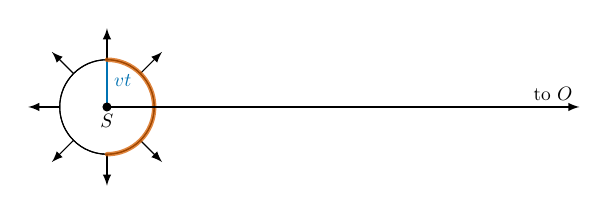
\begin{tikzpicture}[every node/.style={scale=0.7}]
%		\node[inner sep=0pt] (russell) at (0,0.05){\includegraphics[scale=0.25]{bilder/aberration2}};

%		\draw [step=.1, gray,thin, opacity=0.5] (-4,-2) grid (4,2);
%		\draw [step=1, black, opacity=0.5] (-4,-2) grid (4,2);
		
		\coordinate (S) at (-2.5, 0);
		
		\draw[-latex] (S) -- (-3.5, 0);
		
		\draw[-latex] (S) -- (-2.5+0.7,  0.7);
		\draw[-latex] (S) -- (-2.5+0.7, -0.7);
		
		\draw[-latex] (S) -- (-2.5-0.7,  0.7);
		\draw[-latex] (S) -- (-2.5-0.7, -0.7);
		
		\draw[-latex] (S) -- (-2.5, 1);
		\draw[-latex] (S) -- (-2.5, -1);
%		
%		\draw[-latex] (S) -- (-1, 1.5);
%		\draw[-latex] (S) -- (-1, -1.5);
%		
%		\draw[-latex] (S) -- (0.9, 1.7);
%		\draw[-latex] (S) -- (0.9, -1.7);
		
%		\draw[-latex] (S) -- (2.4, 1);
%		\draw[-latex] (S) -- (2.4, -1);
		
		
		
		\draw[fill=white] (S) circle (0.6);
		
		\draw[MyBlue, line cap=round, thick] (S) -- (-2.5, 0.6) node [right, pos=0.55] {\( v t \)};
		
		\draw (S) circle (0.6);
		
		\draw[ultra thick, MyOrange, opacity=0.75, line cap=round] (-2.5, -0.6) arc (-90:90:0.6);
		
		\draw[fill] (S) circle (0.05cm) node [below] {\( S \)};
		
		\draw[-latex] (S) -- (3.5, 0) node [above left] {to \( O \)};
	\end{tikzpicture}
	
	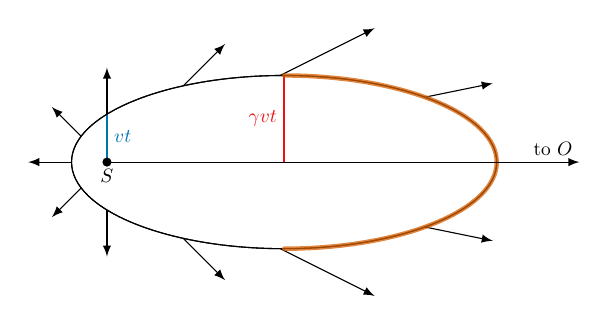
\begin{tikzpicture}[every node/.style={scale=0.7}]
%		\node[inner sep=0pt] (russell) at (0,0.05){\includegraphics[scale=0.25]{bilder/aberration2}};
		
%		\draw [step=.1, gray,thin, opacity=0.5] (-4,-2) grid (4,2);
%		\draw [step=1, black, opacity=0.5] (-4,-2) grid (4,2);
		
		\coordinate (S) at (-2.5, 0);
		
		\draw[-latex] (S) -- (-3.5, 0);
		
		\draw[-latex] (S) -- (-3.2, 0.7);
		\draw[-latex] (S) -- (-3.2, -0.7);
		
		\draw[-latex] (S) -- (-2.5, 1.2);
		\draw[-latex] (S) -- (-2.5, -1.2);
		
		\draw[-latex] (S) -- (-1, 1.5);
		\draw[-latex] (S) -- (-1, -1.5);
		
		\draw[-latex] (S) -- (0.9, 1.7);
		\draw[-latex] (S) -- (0.9, -1.7);
		
		\draw[-latex] (S) -- (2.4, 1);
		\draw[-latex] (S) -- (2.4, -1);
		 
		 
		
		\draw[fill=white] (-0.25,0) ellipse (2.7 and 1.1);
		
		\draw[MyBlue, line cap=round, thick] (S) -- (-2.5, 0.6) node [right, pos=0.55] {\( v t \)};
		\draw[MyRed, thick] (-0.25, 0) -- (-0.25, 1.1) node [left, pos=0.5] {\( \gamma v t \)};
		
		\draw (-0.25,0) ellipse (2.7 and 1.1);
		
		\draw[ultra thick, MyOrange, opacity=0.75, line cap=round] (-0.25,0) [partial ellipse=-90:90:2.7 and 1.1];
		
		\draw[fill] (S) circle (0.05cm) node [below] {\( S \)};
		
		\draw[-latex] (S) -- (3.5, 0) node [above left] {to \( O \)};
		
	\end{tikzpicture}
\end{document}